\chapter{Software}
\label{sec:Software}
\pagestyle{scrheadings}
\section{DAVE Entwicklungsumgebung}

Das Programm DAVE (Digital Application Virtual Engineer) wird von Infineon Technologies AG entwickelt. Es basiert auf der Entwicklungsumgebung oder \ac{IDE} \enquote{eclipse} die von der Eclipse Foundation entwickelt wird. Eine \ac{IDE} beschreibt dabei allgemein ein Programm zur Softwareentwicklung, welches die einzelnen dazu notwendigen Tools gesammelt zur Verfügung stellt. Dies sind vor allem der Compiler, der Linker, und der Debugger auf die im folgenden noch eingegangen werden soll. DAVE stellt eine Möglichkeit zum Editieren von Quelltexten und Anordnen der einzelnen Programmdateien bereit. Über den enthaltenen GNU C-Compiler wird der erstellte Quellcode in vom XMC lesbare Maschinensprache übersetzt und anschließend durch den Linker zu einem ausführbaren Programm vereint. Durch den enthaltenen Debugger kann das Programm in den Speicher des XMC geladen werden. Dort kann der Programmablauf gestartet und gestoppt werden, außerdem können Werte einzelner Register und Variablen ausgelesen werden. 
%cite c als erste prog sprache

DAVE greift bei der Programmierung von Mikrocontrollern der XMC-Serie auf die so genannten XMC Libraries zurück, die von Infineon ebenfalls zur Verfügung gestellt werden.  Auf diese soll ebenfalls im weiteren Verlauf  eingegangen werden. Ein weiteres Feature in der \ac{IDE} sind die sogenannten DAVE APPs. Mit diesen soll die Programmierung des Mikrocontrollers durch ein \ac{GUI} ermöglicht werden. Dazu werden für  mögliche, von der Hardware zu verrichtende Teilaufgaben, APPs von Infineon bereitgestellt. Durch das Einfügen der entsprechenden APPs in das Projekt können diese angepasst und miteinander grafisch verschalten werden. So wird der spätere Programmablauf im Mikrocontroller und dessen Aufgaben festgelegt. Nachdem vom Programmierer noch die Pins ebenfalls grafisch den Aufgaben zugeordnet werden, generiert  DAVE  den Programmcode mit den in den Apps enthaltenen Informationen%\cite{DAVEQuickStart}.
Mithilfe des DAVE \ac{SDK} können nicht nur die Parameter der APPs beim Programmieren , sonder auch diese selbst grundlegend angepasst werden und das Entwickeln eigener APPs ist möglich%\cite{DAVE-Version-4}.

Im Verlauf dieser Arbeit wurden DAVE  APPs jedoch nur in einem bereits existierenden Softwareprojekt für ein Relax Kit genutzt, mit welchem  Signale zum Testen der Empfänger an die Basisstation gesendet wurden. In der Basisstation selbst wurden die APPs\index{APP} jedoch nicht benutzt.


\section{verwendete Peripherie des XMC4500}


Der XMC4500-Baustein enthält diverse funktionelle Blöcke, die mit einer Bus Matrix an die ARM Cortex-M4 \ac{CPU} angebunden sind. Dieser Aufbau soll den Prozessor entlasten und im Programmablauf Ressourcen freihalten für andere Operationen.%System Block Diagram aus Datenblatt einfügen und zitieren
Für die Basisstation waren vor allem der \acs{USIC}, der \ac{USB} sowie der \ac{ETH} die bedeutende Peripherie. Von besonderer Bedeutung sind jedoch die \acp{GPIO}. %wird plural richtig gebildet?






\subsection{GPIO}
Die \acp{GPIO} werden im so genannten PORTS-Modul der XMC-Architektur gesteuert. In dieser lassen sich die Treiberstufen für die entsprechenden Pins des Mikrocontroller regeln. Dieses Modul ist über die Peripheriebrücke PBA1 ebenfalls an die Bus Matrix \index{Bus Matrix} und somit den Cortex-M4 Kern angebunden.  %Programmable port driver control module (PORTS) Abkürzung richtg?dann einfügen
%Bild StructureDigitalPin einbinden
%beschreiben wie pins belegt sind, wann GPIO bzw wann module (s. Pinbelegung) auf Pins liegen ( bei POSIF Kapitel beschreiben

Das Modul stellt für jeden Pin die erste Funktionsauswahl bereit und legt so die Datenrichtung fest. Im \enquote{Port Input/Output Control Register} des Moduls wird für jeden Pin festgelegt, ob er als Eingang oder Ausgang verwendet wird. Das momentane elektrische Potential am Eingang wird bei letzterem mit einem Schmitt-Trigger in ein binäres logisches Signal übersetzt. Ist der Pin ein Eingang, so kann das logische Eingangssignal dort zusätzlich invertiert werden. Wird ein Pin des XMC als Ausgang konfiguriert, so kann gesteuert werden, ob es sich um einen \ac{GPIO}-Pin handelt, dessen Status von der Software direkt festgelegt wird. Dabei kann ausgewählt werden, ob das logische Ausgangssignal durch einen Treiber in Open-Drain Konfiguration oder durch Push-Pull erzeugt werden soll. 

Zur Nutzung eines Ausgangs durch die im Mikrocontroller verfügbaren Peripherie sind diese direkt mit den entsprechenden Modulen verbunden. Dadurch kann das Modul selbst den elektrischen Zustand am Eingang auslesen und verwerten oder festlegen wenn es sich um einen Ausgang handelt \cite{XMC-Reference}. 
Auch das weitere Verhalten von Pins, wie etwa  beim Anschalten, bevor die Versorgungsspannung ein gültiges Level erreicht hat, lassen sich im PORTS-Modul anpassen.
\begin{figure}[h]
	\centering
	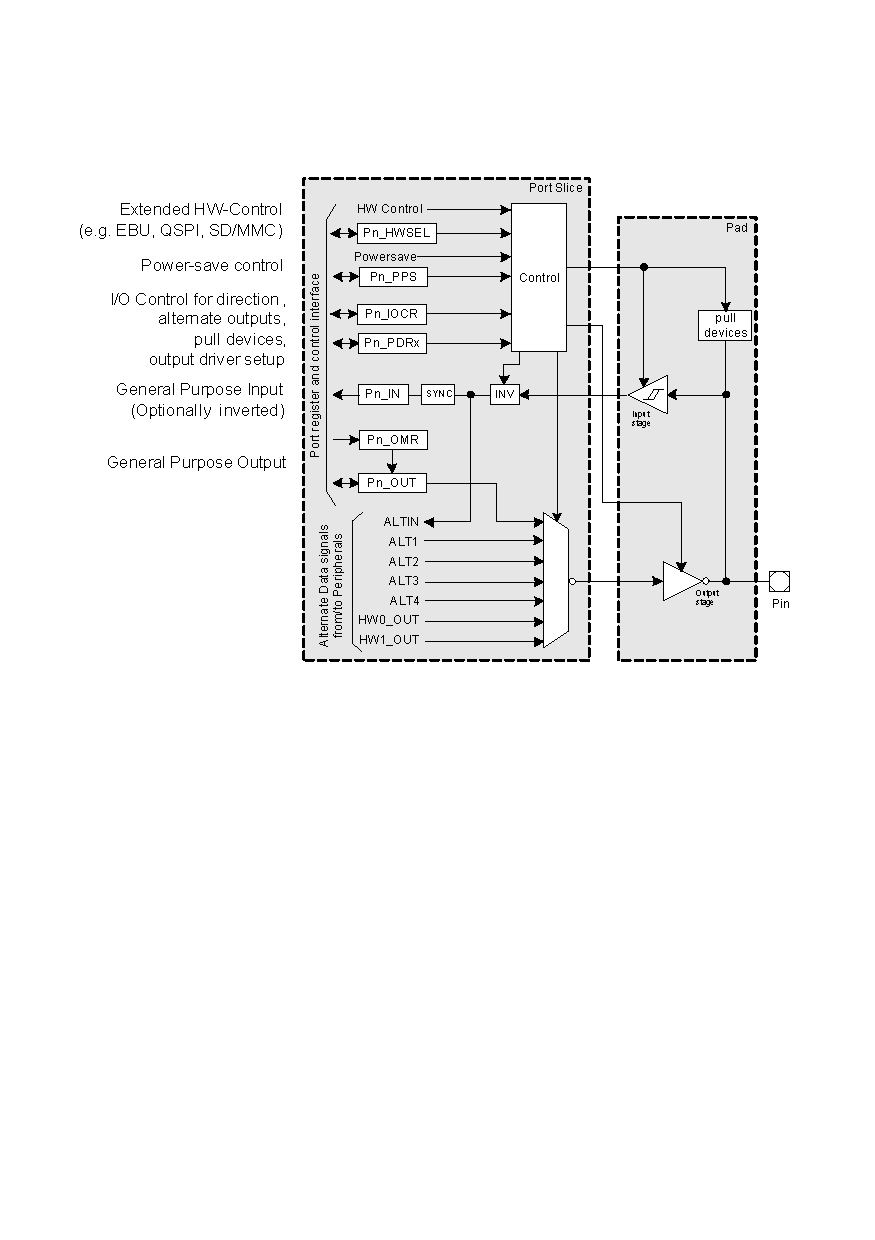
\includegraphics[width=0.7\linewidth]{Abbildungen/StructureDigitalPin}
	\caption{Struktur eines Digitalpins des XMC Mikrocontroller. aus \cite{XMC-Reference}}
	\label{fig:structuredigitalpin}
\end{figure}


\subsection{USIC}
Die \acp{IC} der XMC-Familie verfügen über ein Modul zu Kommunikation über diverse serielle Protokolle, den \acf{USIC}. Dieses ist programmierbar und erlaubt damit eine individuelle Verwendung, kann aber gleichzeitig die notwendigen Arbeiten für den Prozessor übernehmen. Der XMC4500 verfügt über insgesamt sechs \ac{USIC}-Kanäle und kann somit mehrere Protokolle gleichzeitig verwenden. Die Mikrocontroller unterstützen die  Protokolle UART, I$^{2}$C, IIS, LIN und das für die Basisstation verwendete SPI in einfacher, doppelter und quad-Ausführung. Für diese Arbeit wurde alle Kommunikation mit einem gemeinsamen \acs{USIC}-Kanal umgesetzt. Da die einzelnen \acp{USIC} und deren Kanäle verschieden viele Slave-Select-Leitungen besitzen, wurde der Kanal $0$ des \ac{USIC} $0$ ausgewählt, nur dieser verfügt über die benötigten sechs Select-Leitungen. Eine Umsetzung mit einem anderen USIC wäre ebenfalls möglich gewesen. Die Wahl des Transceivers hätte dann aber manuell erfolgen müssen und hätten nicht vom das Modul geregelt werden können.
%beschreiben Funktion
%wo SPI allgmein beschreiben


\subsection{ERU}
Von zentraler Bedeutung für die Funktion der Basisstation war die Behandlung von Interrupts durch den  \ac{IC}. Der XMC4500 besitzt dafür zwei entsprechende \ac{ERU}-Module, die einen solchen erkennen können und den Prozessor zum Aufrufen einer \ac{ISR} auffordern können. Jedes Modul verfügt über vier Kanäle, auf denen  bei einem Interrupt ein vierstufiger Prozess durchlaufen wird: In der ersten Stufe der \ac{ERU}, der so genannten \ac{ERS}, lassen sich aus zwei Eingängen mit jeweils vier Signalen die gewünschten Eingänge wählen. In der \ac{ETL} generiert der \ac{IC} aus dem Signalstatus ein Trigger-Event, indem Veränderungen erkannt werden. So kann eine fallende oder steigende Flanke, die einen Interrupt auslösen soll, erkannt werden. In der Cross Connection Matrix können Signale der verschiedenen \acp{ETL} zu den vier \acp{OGU} weitergeleitet und somit dort untereinander und mit Triggersignalen von anderen Peripherie-Modulen des XMC kombiniert werden.  In der \ac{OGU} wird durch Vergleich der verschiedenen aufgetretenen Trigger und Muster entschieden, ob ein kompletter Interrupt aufgetreten ist und leitet diese Information entsprechend weiter oder ob etwa nur das gewählte Muster erkannt wurde, was für andere Module wichtig ist. Diese Informationen werden entsprechend an die Peripherie weitergeleitet, sind aber für die Funktion der Basisstation nicht weiter von Bedeutung. 
Bei Vorliegen aller Bedingungen für einen Interrupt wird diese Information an den \ac{NVIC} im Cortex-M4 weitergeleitet. Dieser Teil des Prozessorkerns erkennt die Interruptaufforderung und sorgt dafür, das der aktuelle Prozessorstatus gespeichert wird. Nach Ablauf der \ac{ISR} wird der Prozessorstatus wieder hergestellt.
%wo falsche wahl der Pins einbringen?
%Interrupt Request, IRQ im gegensatz zu isr https://de.wikipedia.org/wiki/Interrupt

\subsection{USB}
Das \ac{USB}-Modul des XMC4500 arbeitet nach den  Spezifikationen für USB 2.0 und den \enquote{On-The-Go}-Spezifikationen der Version 1.3. Der Mikrocontroller könnte durch das \ac{USB}-Modul sowohl als Host oder als USB-Slave  arbeiten. In diesem Fall wurde der \ac{IC} als Slave betrieben. Das \ac{USB}-Modul verfügt über eine eigene Interruptsteuerung und ist damit eine der oben erwähnten Peripherien des XMC, deren Steuerung auch über Interrupts gelöst ist. Die gesamte Übertragung wird durch den \ac{USB}-Kern gesteuert und empfangene oder zu sendende Pakete werden in einem \ac{FIFO}-Puffer gespeichert. Für die Kommunikation der Basisstation mit dem Host-Computer wird ein virtueller COM-Port durch das \ac{USB}-Interface emuliert.

\subsection{Ethernet} 
Im XMC4500 werden Netzwerkverbindungen durch das  Ethernet-Modul behandelt. Dieses unterstützt Datenübertragungen mit Geräten über IPv4 und IPv6 sowie Übertragungsraten von \unit[10/100]{MBit/s}.  Dazu werden zunächst die Daten von der CPU über ein Bus-Interface übertragen. Im \enquote{MAC Transaction Layer} werden die vom Prozessor bzw. über Ethernet empfangenen Datenpakete zwischengespeichert. Der Ethernet-Kern formatiert die zu sendenden Daten und stellt sie einem \enquote{Physical Layer} zu, welches die Daten für den Kanal moduliert.






\section{verwendete Bibliotheken}
\subsection{XMC Library (XMC Lib)}
Infineon stellt für seine \acp{IC} der XMC4000 Serie, zu der auch der XMC4500 gehört, die \enquote{XMC Peripheral Library} bereit. Diese erlaubt einen vereinfachten Zugriff auf alle Module und die entsprechenden Register und soll dadurch den Modulzugang übersichtlich gestalten und den Programmcode vereinfachen und leichter lesbar machen. Die Software baut auf dem \ac{CMSIS} auf, erlaubt die Verwendung verschiedener Compiler und kann kann mit oder ohne DAVE bzw. mit oder ohne DAVE APPs verwendet werden. %C99 usage +  weiter beschreiben etc
Für die Programmierung wurde mit der Software \enquote{doxygen} eine Dokumentation zur Bibliothek als HTML generiert.

\subsection{SPI Library}
Die verwendete Bibliothek zur Steuerung des \ac{SPI}-Interfaces basiert auf dem \ac{SPI}-Modul der XMC Library. Die von Infineons XMC Library zur \ac{SPI}-Kommunikation zur Verfügung gestellten Funktionen steuern das \ac{USIC}-Modul des Mikrocontrollers an. Die Bibliothek zur \ac{SPI}-Kommunikation muss somit nur noch die Funktion
\begin{lstlisting}
XMC_SPI_CH_Transmit(channel, data, XMC_SPI_CH_MODE_STANDARD);
\end{lstlisting} der XMC Library aufrufen, um eine Übertragung über das Serielle Interface durchzuführen. Daneben liegt die Hauptaufgabe der Bibliothek vor allem in der der Auswahl des entsprechenden Transceivers über das Slave-Select-Signal. Dazu initalisiert die Bibliothek zuerst den \ac{USIC} entsprechend den in der Headerdatei vorgegebenen Pins für MISO, MOSI und den Pins zur Auswahl des jeweiligen Slaves.

\subsubsection*{SPI Übertragung}
%todo: verschieben?
Die durch die Software umgesetzte serielle Übertragung zwischen den \acp{IC} entspricht dem \ac{SPI}-Protokoll, das ursprünglich von Motorola entwickelt wurde\cite{BuchSPI}. Durch das Chip Select–Signal wählt der XMC den entsprechenden Transceiver aus. Da der TDA5340 active-Low arbeitet, also bei anliegendem \ac{GND}-Potential als ausgewählt gilt, wird dieser Eingang im Datenblatt auch als \acf{NCS} bezeichnet. 
Der \ac{USIC} des XMC beginnt nun die Clockleitung des Busses zu treiben. Eine Periode dieser zyklischen Rechteckspannung begrenzen dabei die Zeit in der das auf den \ac{MOSI} und \ac{MISO}-Leitungen ein Bit übertragen wird. Dabei stellt nach der Definition aus dem Datenblatt des Transceivers ein \unit[0]{V}-Spannungspegel eine logische $0$ dar. In der Kommunikation mit den TDA5340 werden jeweils acht Bit zu einem Datenwort zusammengefasst. Der Transceiver erwartet mit dem ersten Datenwort eine Instruktion und je nach Art dieser noch einen Parameter durch die Übertragung des folgenden Wortes. Mögliche Anweisungen sind dabei das Lesen oder Schreiben eines Registers dessen Adresse als Parameter übertragen wird, das Auslesen oder Beschreiben der \ac{FIFO}-Speicher oder das Setzen des TDA5340 in den so genannten \enquote{Transparent Mode} auf den nicht weiter eingegangen werden soll. Nach Übertragung von Instruktion und Parameter werden entweder vom Master oder vom Slave, also vom Transceiver, die gewünschten Daten übertragen.

Beim Schreibzugriff auf den TDA kann durch geeignete Instruktion gewählt werden ob nur auf ein Register geschrieben wird oder ob der Transceiver nachfolgende Datenwörter als Werte in die folgenden Register übernehmen soll. 
Beim Lesezugriff besteht die selbe Auswahlmöglichkeit. Bild \ref{fig:spistart} zeigt den Start einer solchen \ac{SPI}-Kommunikation zwischen dem Transceiver TDA1 und dem Mikrocontroller. Die Dauer der Übertragung betrug etwa \unit[0,26]{ms}. Bei dieser wurde die Instruktion \enquote{Read from Chip}, dargestellt durch den Hexadezimalwert 0x03 und die Registeradresse 0xD3 als Parameter vom Mikrocontroller zum Transceiver übertragen. Dieser teilt durch das folgende Datenwort auf der \ac{MISO}-Leitung, in diesem Fall 0xFF den aktuellen Wert des Registers mit. Der Master beendet daraufhin die Kommunikation durch einen High-Pegel an der Select-Leitung


\begin{figure}[h]
\centering
\includegraphics[width=\linewidth]{"Abbildungen/Aufnahmen/Bilder/Logic Analyser/SPI_Start"}
\caption{Start einer SPI-Übertragung zwischen dem Mikrocontroller und dem Transceiver}
\label{fig:spistart}
\end{figure}


\subsection{TDA5340 Library}
Die Hauptaufgabe in der Kommunikation mit den Transceiver-\acp{IC} wurde durch die vorgegebene Bibliothek für den TDA5340 übernommen. Diese stellte Funktionen zum Senden und Empfangen von Daten mit dem Transceiver zur Verfügung. Die Bibliothek liest dazu den Empfangs-\ac{FIFO} aus oder schreibt in den Puffer für zu sendende Daten. Auch der Lese- und Schreib-Zugriff auf die Steuerregister der Transceiver kann über die Bibliothek geregelt werden. Dazu stellt die Bibliothek auch entsprechende Makros bereit, welche die Namen der Register in die hexadezimale entsprechende Adresse umwandeln, was die Lesbarkeit erheblich beeinflusst. Daneben wurde über die Bibliothek auch die notwendigen  Einstellungen für das Erkennen von Interrupt im XMC4500 vorgenommen. In diesem Bereich waren die notwendigen Anpassungen der Library am tiefgreifendsten, da diese nur für die Interruptbehandlung mit einem Transceiver ausgelegt war. Bei anderen Funktionen der Bibliothek waren nur kleinere Anpassungen notwenig, sodass etwa sichergestellt wurde, für welchen Transceiver die aufgerufene Funktion ausgeführt werden sollte, etwa bei welchem das entsprechende Register ausgelesen wurde.
Zur Verbindung mit den TDA5340 basierte die Bibliothek auf der SPI Library. Dieser wurde die Nummer des Transceivers als Chip-Select übergeben um sicherzustellen, das mit dem richtigen kommuniziert wurde.


\subsection{Virtueller COM Port}
Die Kommunikation der Basistation mit dem Hostcomputer zum Übertragen der gemessene Werte wurde nach dem Vorbild eines Beispielprojektes für DAVE umgesetzt. Die Bereitstellung des virtuellen seriellen Ports erfolgt auf Seiten des XMC über die LUFA (Lightweight USB Framework for AVRs)-Bibliothek. Mit dieser beschränkt sich die Ausgabe über den COM-Port auf das Übergeben der zu sendenden Zeichen an eine entsprechende Funktion. Eine Steuerung des XMC durch Empfangen von Daten über den COM-Port wäre mit der Bibliothek ebenfalls möglich, war jedoch nicht notwendig.
Die Bibliothek und das Beispielprojekt wurde dahingehend angepasst, dass ganze Zeichenketten statt nur einzelner Zeichen der Funktion zum Senden übergeben werden konnten. Auch wurde das Senden von Integer-Variablen ermöglicht, indem diese zu Zeichen umgewandelt wurden. Dabei wurde der \ac{ASCII} beachtet, nach dem die Übertragung funktioniert. So benötigt der COM-Port zur Ausgabe der Ziffer $1$ den dezimalen Wert $49$ nach der Vorgabe durch den \ac{ASCII}-Code.


\section{Programmablauf}
Im Programmablauf des XMC wurde zunächst eine Warteschleife umgesetzt, in welcher der Mikrocontroller auf eine erste Eingabe durch den Benutzer am Hostcomputer wartet. Bereits hier wurde die Übertragung über den seriellen COM-Port initialisiert. Nachdem diese Bestätigung über den COM-Port vom Mikrocontroller empfangen wurde setzt dieser zunächst alle Transceiver in den Schlafmodus, von welchem aus eine Kommunikation möglich ist. Daraufhin beginnt der XMC4500 mit der Konfiguration der für die Interrupts notwendigen Pins und ermöglicht somit das Empfangen von \acp{IRQ} durch die TDA5430. Anschließend initialisiert er zunächst das SPI-Modul, um im folgenden die Transceiver darüber konfigurieren zu können. Bevor das dazu notwendige Schreiben in die Register der TDAs jedoch möglich ist, wird eine gewisse Verzögerung benötigt. Diese resultiert daher, dass der Wechsel des TDA vom ausgeschalteten Zustand in den Schlafmodus eine gewisse Zeitspanne benötigt. 
Im folgenden werden alle Transceiver initialisiert und anschließend in den Receiver-Modus gefahren.  
Daraufhin setzt der \ac{IC} noch alle für die Übertragung notwendigen Variablen  und alle Felder zum Speichern von Daten zu null. 
Nun beginnt der Prozessor mit einer Dauerschleife, in der dieser auf das Ankommen von Übertragungen wartet und teilt dies auch dem Benutzer am Hostcomputer über eine Ausgabe mit. In dieser Endlosschleife wechselt sich die interruptbasierte Datenerfassung mit der Weiterleitung der erfassten Daten zyklisch ab, wobei nur bei erfolgreichem Empfang ein Senden an den steuernden Computer erfolgt. 

%TODO:genauer alles?!; wo beschreiben? 

Bei der Programmierung wurde darauf geachtet möglichst alle Konstanten wie Adressen von Pins und Ports durch Makros für den Präprozessor auszulagern. Dadurch konnte einerseits die Lesbarkeit des Quellcodes erhöht werden, andererseits sind so aber Änderungen durch vertauschen von Pins, sowohl in der Hardware als auch nur in Software, leichter möglich. Da es sich beim XMC4500 um einen Mikrocontroller mit einer 32Bit Architektur handelt wurden Integervariablen ausschließlich vom Typ \textit{uint32\_t} oder \textit{int32\_t} verwendet. So konnte eine genaue Anpassung der Software an die Registergrößen im XMC vorgenommen werden.



\subsection{Konfiguration der Funkmodule}

Bei der Initialisierung erhalten die Transceiver die gewünschten Werte für die Sende- und Empfangs-Frequenzen. Diese werden über die Teilerrate für die  \ac{PLL} übergeben und ermittelt. Über die entsprechenden Register wird auch das Verhalten bei ankommenden Übertragungen eingestellt. Der TDA5340 stellt dafür mehrere Konfigurationssätze zur Verfügung in denen unterschiedliche Frequenzen eingestellt werden können. In diesem Fall wird zum Empfangen die Konfiguration A und Konfiguration B zum Senden eingestellt. Die entsprechenden Werte wurden zuvor aus der Zwischenfrequenz  $f_{IF2}=\unit[274]{kHz}$ und der gewünschten Übertragungsfrequenz errechnet.


Im \enquote{Interrupt Mask}-Register wurde eingestellt bei welchen Ereignissen der Transceiver einen solchen auslösen wird. Zur Ausgabe dieser wurde der standartmäßige PP2-Pin des Transceivers verwendet. PP1 und PP0 wurde in einen hochohmigen Zustand versetzt, da diese zum aktuellen Zeitpunkt nicht genutzt wurden.
 
 
 
 
%und rechnung aus exekl sheet einfügen


%TODO hier  fehlt etwas


\subsection{Interruptbasierte Datenerfassung}


Die Erfassung der Daten erfolgt im Programmablauf innerhalb der dauerhaften Ablaufschleife.
In der \acf{ISR}, in welche der Prozessor beim Auftreten eines Interrupts springt, wird lediglich einer globalen Variable der Wert $1$ zugeordnet. Für jeden der möglichen Transceiver existiert eine solche Flagge, die einen aufgetretenen Interrupt anzeigt. Nach dem Setzen in der \ac{ISR} kehrt der Prozessor zum Ablauf in die Dauerschleife zurück. Innerhalb dieser wird nun zyklisch abgefragt, ob diese Flagge gesetzt wurde. Beim Auftreten einer solchen Flagge, also nach dem aufgetretenen Interrupt, liest der XMC4500 die  Interrupt Status Register des entsprechenden Transceivers aus. 
Da davon auszugehen ist, das alle sechs Transceiver-\acp{IC} zeitgleich eine Übertragung erhalten, wurde diese mehrstufige Abfrage gewählt. So wird zuerst nur in der \ac{ISR} die Flagge gesetzt, um die dadurch verstreichende Zeit möglichst kurz zu halten und zu ermöglichen, dass eine solche Flagge auch jederzeit im Programmablauf gesetzt werden kann. In der zweiten Stufe liest der Mikrocontroller nun die drei Interrupt Status Register aus. Dies ist notwenig, da es sich dabei um so genannte \enquote{Read-Clear}-Register handelt, welche  nach dem Auslesen über SPI automatisch zurückgesetzt werden.
In den Interrupt-Registern sind die Ereignisse kodiert, die einen Interrupt ausgelöst haben. Bei der Konfiguration der Funkmodule wurde eingestellt bei welchen Ereignissen der Transceiver einen Interrupt auslöst. Typische Ereignisse sind ein fast gefüllter Empfangs-\ac{FIFO} was eine angekommene Übertragung anzeigt oder auch ein leerer \ac{FIFO} was anzeigt, das dieser ausgelesen wurde. 
Die dritte Stufe  der Datenerfassung ist nun die Abfrage der Daten vom Transceiver. Da diese \ac{SPI}-Datenübertragung deutlich mehr Zeit in Anspruch nimmt, muss diese getrennt vom Erkennen der Interrupts und dem Auslesen der Interrupt-Register erfolgen. Da die gewünschten Werte in den Registern gespeichert sind, ist das Auslesen zeitkritisch, denn eine erneute Übertragung würde diese Messwerte überschreiben. Jedoch ist das Auslesen der Werte bei weitem nicht so zeitkritisch wie die ankommenden Interrupts, da diese im Verlauf einer Übertragung auch mehrfach ankommen können. Das Abfragen der empfangenen Daten aus dem \ac{FIFO}-Speicher hat eine noch geringere Priorität, da dieser die Datenpakete bis zum Auslesen behält. Eine Abfrage der Messwerte und ein Auslesen des \ac{FIFO} wird bei abgeschlossener Übertragung durchgeführt, diesen Zeitpunkt erkennt der Mikrocontroller durch das entsprechend gesetzte Bit des Interrupt-Register. Der XMC4500 speichert alle abgefragten Werte wie Feldstärke, die Einstellungen der \ac{AGC} und die angekommenen Daten in den vorbereiteten dedizierten Speichern. Abschließend werden die Transceiver wieder in den Empfangsmodus gesetzt. 

Beim Setzen der Flaggen durch den Interrupt fiel auf, das die Interrupteingänge für Transceiver 3 und Transceiver 6 sich überlagern. So ist der PP2 Anschluss des dritten TDA5340 mit der \ac{ETL}3 der \ac{ERU}0 verbunden, ebenso wie der entsprechende Pin des TDA6. Grund dafür ist, die entsprechenden Pins dem Mikrocontroller auf dem Kanal B3 bzw. A0 der genannten \ac{ERU}-\ac{ETL}-Kombination führen. Bei den ersten Tests von Interrupts auf diesen Kanälen stellte sich heraus, das der XMC, entgegen der Erwartungen, somit nicht in der Lage ist ankommende Interrupts der beiden Transceiver zu unterscheiden. Durch entsprechende Einstellungen in der \ac{ERU}0 war ein Sprung des Prozessors in die entsprechende \acl{ISR} nur für jeweils einen der beiden Transceiver möglich. Um trotzdem eine Auslesen der beiden Transceiver zu bewirken, wurden beide Flaggen in der Service Routine gesetzt.

Der Versuch den PP2 Pin des TDA6 mittels eines kurzen Drahtes auf den Pin 142 des XMC4500 zu legen schlug ebenfalls fehl. Dazu wurde der PP1 Pin des TDA1, welcher mit diesem Pin des Mikrocontroller verbunden ist im Transceiver 1 in einen hochohmigen Zustand geschaltet. Dieser Pin des XMC ist intern mit der \ac{ETL}2 der \ac{ERU}0 auf dem Kanal B3 verbunden. Da diese Kombination noch nicht verwendet wurde hätte hier eine Interrupterkennung funktionieren müssen. Warum durch diese Veränderung kein Interrupt ausgelöst werden konnte ist nicht klar. Da in der Betrachtung mit dem Logic-Analyser keine Flanke auf dem Netz festgestellt wurde, ist zu vermuten, dass das Problem aus der Verbindung mit dem Draht resultiert.
%unterscheidung der zwei interruptabfragen
%was steht in den registern drinnen und wird abgefragt



\subsection{Weiterleitung der erfassten Daten}
Dass eine Übertragung über den COM-Port bereits weit vor der Dauerschleife vom Mikrocontroller gestartet wurde, diente dazu, dem Benutzer  die Bereitschaft zum Empfangen mitzuteilen sobald sämtliche Initialisierungen abgeschlossen waren. Somit musste der COM-Port auch nun nicht mehr selbst initialisiert werden.
Im zweiten Teil der Ablaufschleife des Programmablaufs wurde nun die Weitergabe der empfangenen Daten und der gemessenen Werte behandelt. Dazu wurde nach dem Abholen der empfangenen Daten von den Transceivern eine Statusflagge in Form einer Integer-Variable gesetzt. Nur beim Auftreten dieser Flagge wurde der Programmteil zum Senden über den COM-Port ausgeführt.
Dort wurde nun jeweils abwechseln ein Wert des Speichers und ein String mit einer Beschreibung oder dem Namen des Wertes über COM ausgegeben. Ein Ausschnitt des Quellcodes ist im Quellcode \ref{listing:COMsend} zu erkennen. Die Zeichenfolge $\backslash r\backslash n$ stellt dabei den Übergang in eine neue Zeile in der Ausgabekonsole dar. Wie in C üblich werden Strings in doppelten Anführungszeichen im Quelltext eingefügt. Eine entsprechende Ausgabe ist in Bild ... zu erkennen. %TODO eingügen referenz
\begin{lstlisting}[caption={Ausschnitt aus dem Senden der Daten über den COM-Port},label={listing:COMsend},captionpos=b,language=C]
COM_send_string("#################### Übertragung erkannt ####################\r\n");
COM_send_string("Übertragung Nummer ");
COM_send_int_as_string(transfernumber);
COM_send_string("\r\n\r\n");
COM_send_string("TDA1:");
COM_send_string("\r\nPMF:");
COM_send_int_as_string(rssiTDA1.pmf);
COM_send_string("\r\nPRX:");
COM_send_int_as_string(rssiTDA1.prx);
COM_send_string("\r\nRX:");
COM_send_int_as_string(rssiTDA1.rx);
COM_send_string("\r\nPPL:");
COM_send_int_as_string(rssiTDA1.ppl);
COM_send_string("\r\nAGC:");
\end{lstlisting}
Am Hostcomputer wurden die Daten mit der Software \enquote{PuTTY} entgegengenommen und dem Benutzer in einer Konsole angezeigt. Dazu wurde der von Infineon zur Verfügung gestellte Treiber verwendet, um dem XMC4500 als COM-Port zu erkennen. %im Anhang/auf CD
Die Einstellungen der Seriellen Übertragung wurden vom Beispielprojekt übernommen, sodass am Computer mit einer Baudrate von \unit[115200]{Bd} und acht Daten Bits pro Zeichen empfangen wurde und was im Programm eingestellt werden musste. Nach der bereits erwähnten anfänglichen Bestätigung der Kommunikation durch den Nutzer, wurden bei jeder vom Mikrocontroller erkannten Übertragung die gemessenen Feldstärkewerte ausgegeben. Neben den PMF, PRX RX, PPL und AGC-Werten wurde noch die Empfangsleistung ausgegeben. Diese wurde zur Laufzeit aus dem PPL und dem AGC-Wert errechnet und in dBm angezeigt. Dazu diente eine vorgegebene Funktion, welche aus dem PPL-Wert und dem Wert der \ac{AGC} mittels kalibrierter Parameter eine Feldstärke berechnete. Die Werte wurden in einem Vorprojekt durch Messungen kalibriert und sind hier nicht weiter von Bedeutung. Die Abkürzungen der übertragenen Werte sind in Tabelle \ref{tab:RSSI} aufgeführt.
\begin{table}[tbh]
	\centering
	\begin{tabular}{ll}
		
		PMF			&Peak Memory Filter\\
		PRX			&Peak Detector\\
		RX			&\acf{RSSI}\\
		PPL			&RSSI Payload Peak Detector\\
		AGC			&Automatic Gain Control\\
		
	\end{tabular}
	\caption{Verwendete Abkürzungen der übertragenen Messwerte}
	\label{tab:RSSI}
\end{table}
Die empfangenen Daten wurden ebenfalls ausgegeben. 
Alle Werte und Daten wurden nach Transceiver getrennt ausgegeben, um eine Vergleichsmöglichkeit zu geben und um die Ausgabe möglichst übersichtlich zu gestalten.
Auch wurden die empfangenen Übertragungen durchnummeriert und die entsprechende Übertragungsnummer mit ausgegeben. So ließen sich einerseits die Sendepositionen den gemessenen Werte zuordnen. Andererseits waren so aber auch  verlorengegangene  Übertragungen sichtbar. Eine typische Ausgabe der Konsole ist im Bild \ref{fig:ConsolePutty} zu erkennen. Zur Darstellung einer eingegangenen Übertragung an der Basisstation sollte die LED Nummer 7 nach jedem Empfangen kurz rot aufblinken. %Bild Übertragung 1 einfügen



%wie viel speicher braucht man aaktuell?